\documentclass[]{report}

\voffset=-1.5cm
\oddsidemargin=0.0cm
\textwidth = 480pt

\usepackage{framed}
\usepackage{subfiles}
\usepackage{graphics}
\usepackage{newlfont}
\usepackage{eurosym}
\usepackage{amsmath,amsthm,amsfonts}
\usepackage{amsmath}
\usepackage{color}
\usepackage{amssymb}
\usepackage{multicol}
\usepackage[dvipsnames]{xcolor}
\usepackage{graphicx}
\begin{document}

	\chapter{Regression}
	
	
	\subsection{Regression Example}
	\begin{itemize}
		\item A study was made by a retailer to determine the relation between weekly advertising
		expenditure and sales (in thousands of pounds).
		\item Find the equation of a regression line
		to predict weekly sales from advertising.
		\item Estimate weekly sales when advertising
		costs are 35,000.
	\end{itemize}
	
	%%%%%%%%%%%%%%%%%%%%%%%%%%%%%%%%%%%%%%%%%%%%%%%%%%%%%%%%%%%%%%%%%%%%%%%%%
	
	\subsection{Regression Example}
	Units denominated in thousands \\(i.e. X = 40 means advertising cost of 40,000)
	\begin{center}
		\begin{tabular}{|c|c|c|c|c|c|c|}
			\hline
			% after \\: \hline or \cline{col1-col2} \cline{col3-col4} ...
			Adv. Costs & 40 & 20 & 25 & 20 & 30 & 50\\
			Sales & 385& 400& 395& 365& 475& 440\\ \hline \hline
			Adv. Costs & 40 & 20 & 50 & 40 & 25 & 50\\
			Sales & 490& 420& 560& 525& 480& 510\\
			\hline
		\end{tabular}
	\end{center}
	
	
	%%%%%%%%%%%%%%%%%%%%%%%%%%%%%%%%%%%%%%%%%%%%%%%%%%%%%%%%%%%%%%%%%%%%%%%%%
	
	\subsection{Regression Example}
	Scatterplot: Indicates a weak positive linear relationship.
	\begin{center}
		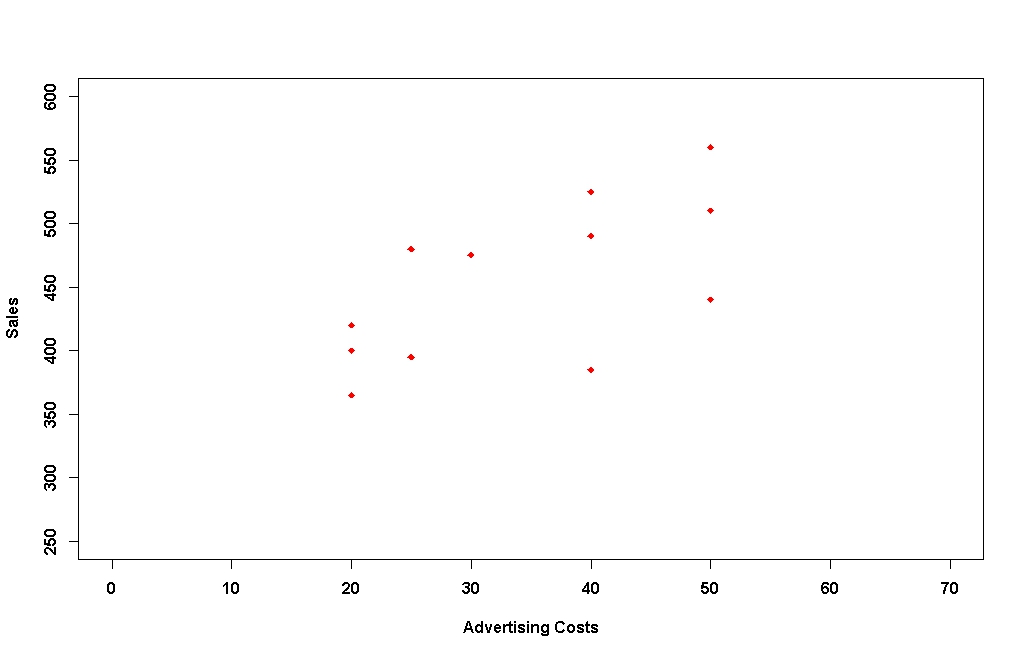
\includegraphics[scale=0.4]{images/12Bplot1}
	\end{center}
	%%%%%%%%%%%%%%%%%%%%%%%%%%%%%%%%%%%%%%%%%%%%%%%%%%%%%%%%%%%%%%%%%%%%%%%%%
	
	\subsection{Regression Example}
	Summations
\begin{multicols}{3}
	\begin{itemize}
		\item $\sum X$ = 410
		\item $\sum Y$ = 5445
		\item $\sum X^2$ = 15650
		\item $\sum Y^2$ = 2512925
		\item $\sum XY$ = 191325
	\end{itemize}
\end{multicols}
	Mean Values
	\begin{itemize}
		\item $\bar{x}$ = 34.16
		\item $\bar{y}$ = 453.75
	\end{itemize}
	
	
	%%%%%%%%%%%%%%%%%%%%%%%%%%%%%%%%%%%%%%%%%%%%%%%%%%%%%%%%%%%%%%%%%%%%%%%%%
	
	\subsection{Regression Example}
	Sums of Squares Identities
	\begin{itemize}
		\item $S_{XX}$ = 1641.67
		\item $S_{YY}$ = 42256.25
		\item $S_{XY}$ = 5287.5
	\end{itemize}
	Pearson's Correlation Estimate
	\[ r_{XY} = \frac{S_{XY}}{\sqrt{S_{XX} \times S_{YY}}} = \frac{5287.5}{\sqrt{1641.67 \times 42256.25}} = 0.6348 \]
	
	Weak to strong positive linear relationship.
	
	%%%%%%%%%%%%%%%%%%%%%%%%%%%%%%%%%%%%%%%%%%%%%%%%%%%%%%%%%%%%%%%%%%%%%%%%%
	
	\subsection{Regression Example}
	Regression Coefficients
	\begin{itemize}
		\item Slope Estimate $b_1$
		\[b_1 = \frac{S_{XY}}{S_{XX}} = {5287.5 \over 1641.67} = 3.221\]
		\item Intercept Estimate $b_0$ = $\bar{y} - b_1 \times \bar{x}$ = $453.75-(3.221\times 34.16)$ = 343.70
	\end{itemize}
	Regression Equation
	\[ \hat{y} = 343.70 + 3.221x \]
	
	
	%%%%%%%%%%%%%%%%%%%%%%%%%%%%%%%%%%%%%%%%%%%%%%%%%%%%%%%%%%%%%%%%%%%%%%%%%
	
	\subsection{Regression Example}
	\begin{center}
		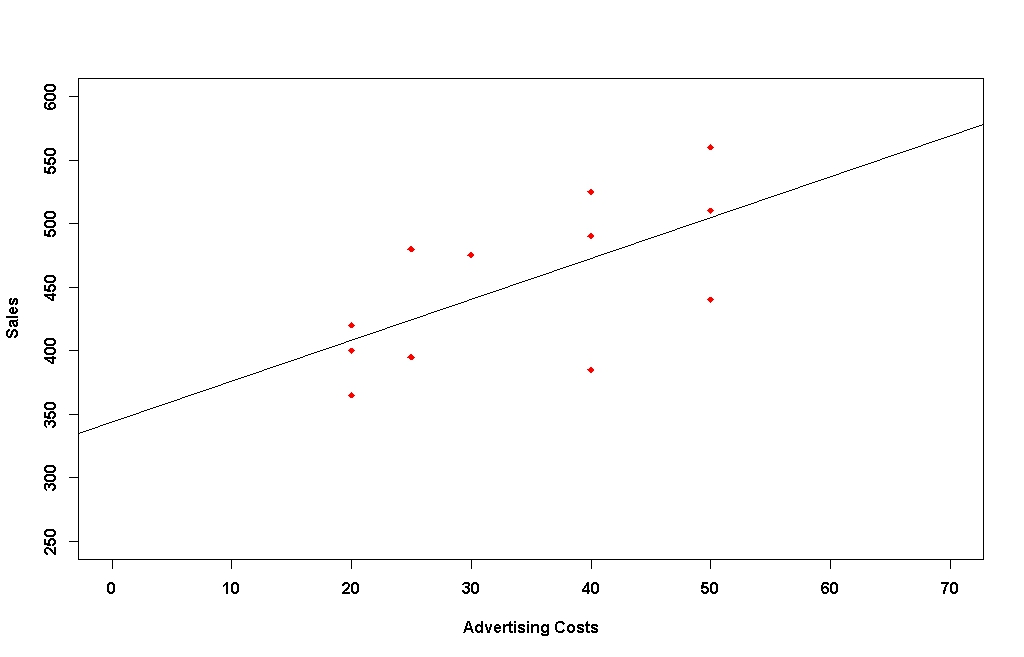
\includegraphics[scale=0.4]{images/12Bplot2}
	\end{center}
	
	%%%%%%%%%%%%%%%%%%%%%%%%%%%%%%%%%%%%%%%%%%%%%%%%%%%%%%%%%%%%%%%%%%%%%%%%%
	
	
	\subsection{Regression Example}
	Estimate weekly sales when advertising costs are 35,000 (i.e X=35).
	\[ \hat{y} = 343.70 + 3.221x \]
	
	\[ \hat{y}_{(X=35)} = 343.70 + 3.221(35)  = 456.4 \]
	
	When the advertising costs are 35,000, the expected sales are predicted to be 456,400.
	
	Estimate weekly sales when advertising costs are 40,000 (ie. X=40).
	
	
	\[ \hat{y}_{(X=40)} = 343.70 + 3.221(40)  = 472.54 \]
	
	When the advertising costs are 40,000, the expected sales are predicted to be 472,540.
	
	
	\subsection{Regression Example}
	
	Predicted and Observed values
	\begin{itemize}
		\item In simple linear regression, we predict scores on one variable from the scores on a second variable.
		\item In the last example, we predicted the value of sales to be 472.54 the costs were X=40.
		\item In fitting the model, we used three observations when the value of X was 40 (i.e. Y = 385,490 and 525)
		\item These are observed values, used to compute the model, and are distinct from predicted values $\hat{y}$.
		\item The predicted values are estimates for future observations
		\item The difference between an observed value and it's corresponding predicted value is known as a \textbf{\textit{residual}}.
		\[e_i = y_i-\hat{y}_i \]
		\item As there are three observations at X=40, there are three residuals.
	\end{itemize}
	
	
	%%%%%%%%%%%%%%%%%%%%%%%%%%%%%%%%%%%%%%%%%%%%%%%%%%%%%%%%%%%%%%%%%%%%%%%%%
	
	\subsection{Regression Example}
	Scatterplot: Indicates a weak positive linear relationship.
	
	\begin{center}
		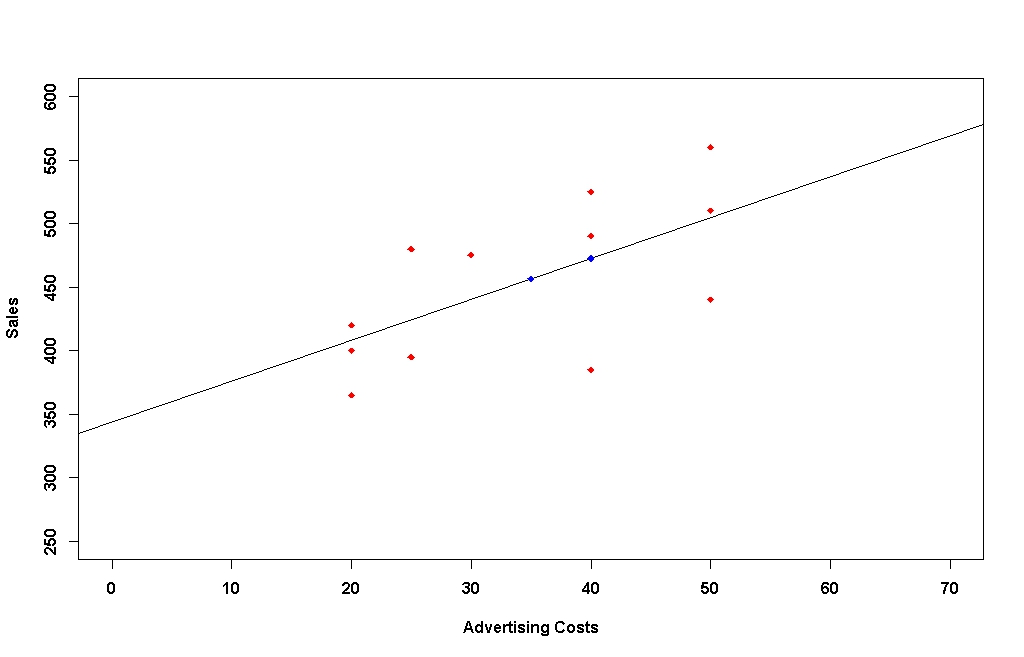
\includegraphics[scale=0.4]{images/12Bplot3}
	\end{center}
	
	
	
	\subsection{Regression Example}
	
	Predicted and Observed Values
	
	\begin{center}
		\begin{tabular}{|c|c|c|c|}
			\hline
			% after \\: \hline or \cline{col1-col2} \cline{col3-col4} ...
			X & Y& $\hat{y}$ & $e_i$ \\
			40 &385 &472.54 &-87.54\\
			40 &490 &472.54 & 17.46\\
			40 &525 &472.54 & 52.46\\
			\hline
		\end{tabular}
	\end{center}
	
	
	
	\subsection{Important Assumptions of Least Squares Regression}
	It is assumed that
	\begin{itemize}
		\item The residuals are independent and normally distributed,
		\item The residuals are normally distributed with mean zero,
		\item The residuals is independent of X.
		\item The variance of residuals is consistent across the range of X (Heteroscedascity).
	\end{itemize}
	If these assumptions are not met, then Least Squares regression is not appropriate as a solution, and other alternatives must be used (Not Part of Course).
	
	%%%%%%%%%%%%%%%%%%%%%%%%%%%%%%%%%%%%%%%%%%%%%%%%%%%%%%%%%%%%%%%%%%%%%%%%%
	
	\subsection{Extrapolation}
	\begin{itemize}
		\item
		Whenever a linear regression model is fit to a group of data, the range of the data should be carefully observed. \item  Attempting to use a regression equation to predict values outside of this range is often inappropriate, and may yield incredible answers. \item This practice is known as extrapolation. \item Consider, for example, a linear model which relates weight gain to age for young children. \item Applying such a model to adults, or even teenagers, would be absurd, since the relationship between age and weight gain is not consistent for all age groups.
	\end{itemize}
	
	
\end{document}